\subsection{16. Автоматы с магазинной памятью (МП-автоматы). Различные варианты определений. Языки, распознаваемые МП-автоматами.}
\Def Автомат с магазинной памятью (МП-автомат) — кортеж $M = \langle Q, \Sigma, \Gamma, \Delta, q_0, F \rangle$, где:

\begin{enumerate}
    \item $Q$ — множество состояний, $Q$ — конечное множество, то есть $|Q| < \infty$;
    \item $\Sigma$ — алфавит, $|\Sigma| < \infty$;
    \item $\Gamma$ — стековый алфавит, $|\Gamma| < \infty$, $\Gamma \cap \Sigma = \varnothing$;
    \item $\Delta \subset \brackets{Q \times \Sigma^* \times \Gamma^*} \times \brackets{Q \times \Gamma^*}$ — множество переходов, $|\Delta| < \infty$;
    \item $q_0 \in Q$ — стартовое состояние;
    \item $F \subset Q$ — множество завершающих состояний.
\end{enumerate}

Переходы имеют вид $\langle q_1, w, \alpha \rangle \rightarrow \langle a_2, \beta \rangle$, $w \in \Sigma^*$, $\alpha \in \Gamma^*$, \textit{то есть когда находимся в состоянии $q_1$, снимаем со стека слово $\alpha$, стек растёт слева направо, читаем слово $w$, переходим в состояние $q_2$, добавляем на стек слово $\beta$.}

\Def Конфигурация МП-автомата $M$ -- кортеж $\langle q, u, \gamma \rangle$, где $q \in Q$, $u \in \Sigma^*$, $\gamma \in \Gamma^*$.

\Def Отношение выводимости $\vdash$ — наименьшее рефлексивное транзитивное отношение, что для любого перехода $\brackets{\langle q_1, u, \alpha \rangle \rightarrow \langle q_2, \beta \rangle} \in \Delta$ выполнено следующее:

\begin{center}
    $\forall v \in \Sigma^*, \eta \in \Gamma^* : \langle q_1, uv, \eta \alpha \rangle \vdash \langle q_2, v, \eta \beta \rangle$
\end{center}

\textbf{Языки, распознаваемые МП-автоматами}

\Def Пусть $M$ — МП-автомат, язык $L \brackets{M}$, распознаваемый МП-автоматом $M$ — множество $\{ w \in \Sigma^* | \exists q \in F : \langle q_0, w, \varepsilon \rangle \vdash \langle q, \varepsilon, \varepsilon \rangle \}$.

\Example Язык правильных скобочных последовательностей распознаётся следующим МП-автоматом:

\begin{center}
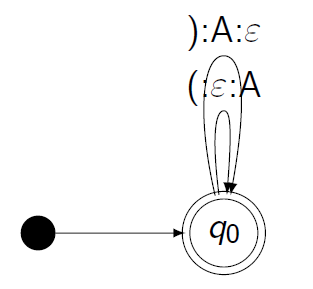
\includegraphics[width=0.25\linewidth]{15_1.png}
\end{center}

\textbf{Упрощения МП-автоматов}

\Statement Для любого МП-автомата существует эквивалентный МП-автомат, для которого выполнено соотношение:

\begin{center}
    $\forall \brackets{\langle q_1, u, \alpha \rangle \rightarrow \langle q_2, \beta \rangle} \in \Delta : |u| \leqslant 1, |\alpha| + |\beta| \leqslant 1$
\end{center}

\Proof

\begin{center}
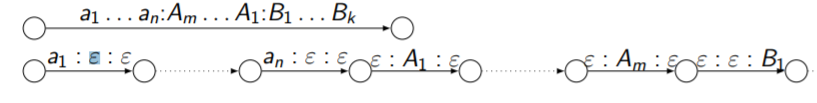
\includegraphics[width=0.85\linewidth]{f2.PNG}
\end{center}

\EndProof

\Statement Для любого МП-автомата существует эквивалентный МП-автомат, для которого выполнено соотношение:

\begin{center}
    $\forall \brackets{\langle q_1, u, \alpha \rangle \rightarrow \langle q_2, \beta \rangle} \in \Delta : |u| \leqslant 1, |\alpha| + |\beta| = 1$
\end{center}

\Proof

\begin{center}
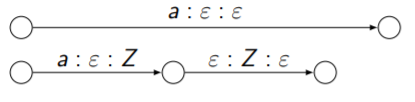
\includegraphics[width=0.65\linewidth]{f3.PNG}
\end{center}

\EndProof
